% !TEX encoding = UTF-8 Unicode
%oneside/twoside for the printer
\documentclass[a4paper,12pt,oneside,final,swedish]{extarticle}
%article vs. extarticle
%Paket
%\usepackage[latin1]{inputenc}	%å,ä,ö
\usepackage[utf8]{inputenc}
\usepackage[T1]{fontenc}
\usepackage{graphicx}
\usepackage{subcaption}
\usepackage{times}			%typsnitt times kanske
\usepackage[swedish]{babel}
\usepackage[affil-it]{authblk}
\usepackage{geometry}	%lets you customize the page size
\usepackage{hyperref}

\geometry{
 margin=20mm
} 

\usepackage{fancyhdr} %include this to customize headers/footers
\usepackage{titling}

%test \paragraph -subsubsub
\makeatletter
\renewcommand\paragraph{\@startsection{paragraph}{4}{\z@}%
            {-2.5ex\@plus -1ex \@minus -.25ex}%
            {1.25ex \@plus .25ex}%
            {\normalfont\normalsize\bfseries}}
\makeatother
\setcounter{secnumdepth}{4} % how many sectioning levels to assign numbers to
\setcounter{tocdepth}{4}    % how many sectioning levels to show in ToC


%-------------------------------------------------------------Här börjar dokumentet 
\begin{document}
% Framsida
\author{Grupp 9\\\\Kalle Bladin\\Erik Broberg\\Emma Forsling Parborg\\Martin Gråd}
\title{Simulering av Elastiska Material}
\clearpage\maketitle %genererar en separat titelsida
\thispagestyle{empty}
\date{2014-03-xx}
\affil{Linköpings Universitet}
\pagebreak
%\pagestyle{empty} %fancy, empty, plain, myheadings




%Sammanfattning
\begin{abstract}
\thispagestyle{empty}
Här ska sammanfattningen skrivas in
\hfill
\end{abstract}
\pagebreak 

%Innehållsförteckning, Figurförteckning & Tabellförteckning
\tableofcontents  % chapter with the table of contents
\addtocontents{toc}{\protect\thispagestyle{empty}}
\listoffigures    % chapter with the list of figures
\addtocontents{lof}{\protect\thispagestyle{empty}}
\listoftables     % chapter with the list of tables
\addtocontents{lot}{\protect\thispagestyle{empty}}

%-----------------------------------------------------------
%Inledning
%\pagestyle{plain}
\pagebreak
\pagestyle{plain}
\setcounter{page}{1}

%Inledning
\section{Inledning}
Inledande text är alltid lite trevligt
\subsection{Introduktion}
  %Syfte
\subsection{Syfte}
Denna rapport syftar till att undersöka hur verklighetstrogna simuleringar av elastiska material kan göras i tre dimensioner med hjälp av mass-fjäder-dämparsystem. 
Simuleringarna som demonstreras är menade att kunna göras i realtid, och erbjuda en användare viss interaktion.

  %Bakgrund
\subsection{Bakgrund}
\subsubsection{Fysikalisk modellering}
En modell som kan användas för simulering av elastiska material är ett så kallat ''mass spring damper system'' (Gelenbe, Lent \& Stakellari 2012) eller MSD-system; en modell som beskrivs av partiklar sammankopplade med fjädrar och dämpare.
\\%Figur
\\Det enkla systemet i Figur X utgör grunden för den struktur som används i detta projekt. 
Genom att utöka systemet med partiklar och samma typ av kopplingar, kan många olika material och former beskrivas, exempelvis tyg, gelé, skumgummi eller liknande elastiska material. 
Beroende på parametrarna fjäderkonstanter, dämparkonstanter, massor och fjäderlängder kan realistiska simuleringar av dessa material uppnås.
\\\\Som bakgrund till den fysikaliska modellen låg de grundläggande rörelse- och kraftlagarna (Halliday 2007) som beskrevs av Newton. 
Newtons andra lag anges i Ekvation 2, 
\\%Ekvation 2
\\där F är den resulterande kraften på en partikel, x?? är partikelns acceleration, m är partikelns massa och t är tidsvariabeln. 
Newtons tredje lag summeras i ett citat:
\begin{quote}''If A puts a force on B, then B puts a force on A, and the two forces are equal in magnitude and have opposite direction.'' (Halliday 2007)\end{quote}
Fjädrarna modellerades med Hookes lag som anges i ekvation 3,
\\%Ekvation 3
\\där F är kraften som fjädern uträttar, k är fjäderkonstanten, l(t) är fjäderns utsträckning, och l0 är fjäderns vilolängd.
\\\\Dämparna modellerades utifrån ekvation 4,
\\%Ekvation 4
\\där F är kraften som dämparen uträttar, b är dämparkonstanten och l är fjäderns utsträckning.
\subsubsection{Numerisk lösning av differentialekvationer}
\subsubsection{Euler}%subsubsub
\subsubsection{Runge Kutta}%subsubsub


%Metod
\section{Metod}
\subsection{Förstudier}
I förstudierna ingick dels framtagandet av en kraftekvation, dels utvecklingen av MSD-system i en och två dimensioner. 
Som verktyg användes MATLAB för att få en visuell återkoppling på kraftekvationen, med hjälp av programmets inbyggda renderingsfunktion.

\subsubsection{Kraftekvation}
\subsubsection{Utveckling av MSD-system}
\paragraph{En dimension}
Då det enkla systemet med två sammankopplade partiklar utökades med fler partiklar och kopplingar, krävdes en mer överskådlig notation för att beskriva systemet. 
I figur \ref{2D_simple} nedan introduceras den nya notationen av ett system med två sammankopplade massor.

\begin{figure}[h!]
  \begin{center}
    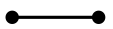
\includegraphics[width=3cm]{Bilder/2D_simple.png} 
  \end{center}
  \caption{Två sammankopplade partiklar}
  \label{2D_simple}
\end{figure}
I MATLAB utvecklades först ett MSD-system i en dimension, där partiklar sammankopplades i serie enligt Figur \ref{simple1D4} nedan.

\begin{figure}[h!]
  \begin{center}
    
\includegraphics[width=6cm]{Bilder/simple1D4.png} 
  \end{center}
  \caption{Fyra sammankopplade partiklar i serie}
  \label{simple1D4}
\end{figure}

Genom att simulera detta system med Euler-metoden samt undersöka hur partiklarnas positioner förändrades över tid, kunde implementationen av den framtagna kraftekvationen enkelt verifieras.

\paragraph{Två dimensioner}
Nästa steg i utvecklingen av MSD-systemet var att implementera det i två dimensioner. 
Detta innebar en övergång från skalärer till vektorer i de framtagna ekvationerna.

För att kunna generera godtyckligt stora MSD-system krävdes en regel för hur partiklarna skulle kopplas ihop med varandra. Två exempel på en partikels möjliga kopplingar visas i Figur \ref{2D_Neighbors} nedan.

\begin{figure}
  \begin{minipage}[b]{.5\linewidth}
    \centering
    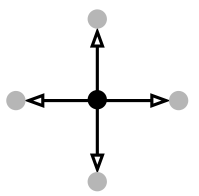
\includegraphics[width=4cm]{Bilder/2D_4Neighbors.png} 
    \subcaption{Partiklar med fyra kopplingar}\label{fig:1a}
  \end{minipage}
  \begin{minipage}[b]{.5\linewidth}
    \centering
    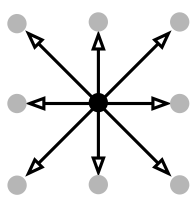
\includegraphics[width=4cm]{Bilder/2D_8Neighbors.png} 
    \subcaption{Partiklar med åtta kopplingar}\label{fig:1b}
  \end{minipage}
  \caption{Två olika sätt att koppla samman partiklar}\label{2D_Neighbors}
\end{figure}

\subsubsection{Indexering av partiklar och kopplingar}
Ett stort problem, som ovanstående stycke implicerar, var att ta reda på vilka partiklar som skulle höra till varje koppling. 
För att detta skulle kunna lösas för godtyckligt stora objekt, behövdes ett systematiskt sätt att tilldela kopplingarna deras partiklar.
Detta löstes med en funktion som utifrån index till en viss koppling gav indexar till de två partiklar som den kopplade samman. 
Genom att låta funktionen genomlöpa alla kopplingar innan simuleringen genomfördes kunde indexeringen användas för att finna de rätta konstanterna (massorna) och variablerna (positionerna och hastigheterna) för de kopplade massorna. 
En liknande funktion implementerades för att finna triangelindexar som användes för renderingen.

\subsubsection{Interaktion med omgivning}
%Algoritm 1: Kollision
\subsubsection{Implementering av kraftekvationen}
%Algorithm 2: baserad på massorna
%Algorithm 3: baserad på kopplingarna mellan massorna
\subsection{Implementering}

\subsubsection{Grundläggande systemarkitektur}
Att övergå till ett objektorienterat system innebar att en systemarkitektur behövde tas fram. 
För att ge en grundläggande förståelse av systemarkitekturen beskrivs denna med ett blockdiagram där de primära modulerna är separerade från varandra. 
Se Figur \ref{systemark}.
\begin{figure}[h!]
  \begin{center}
    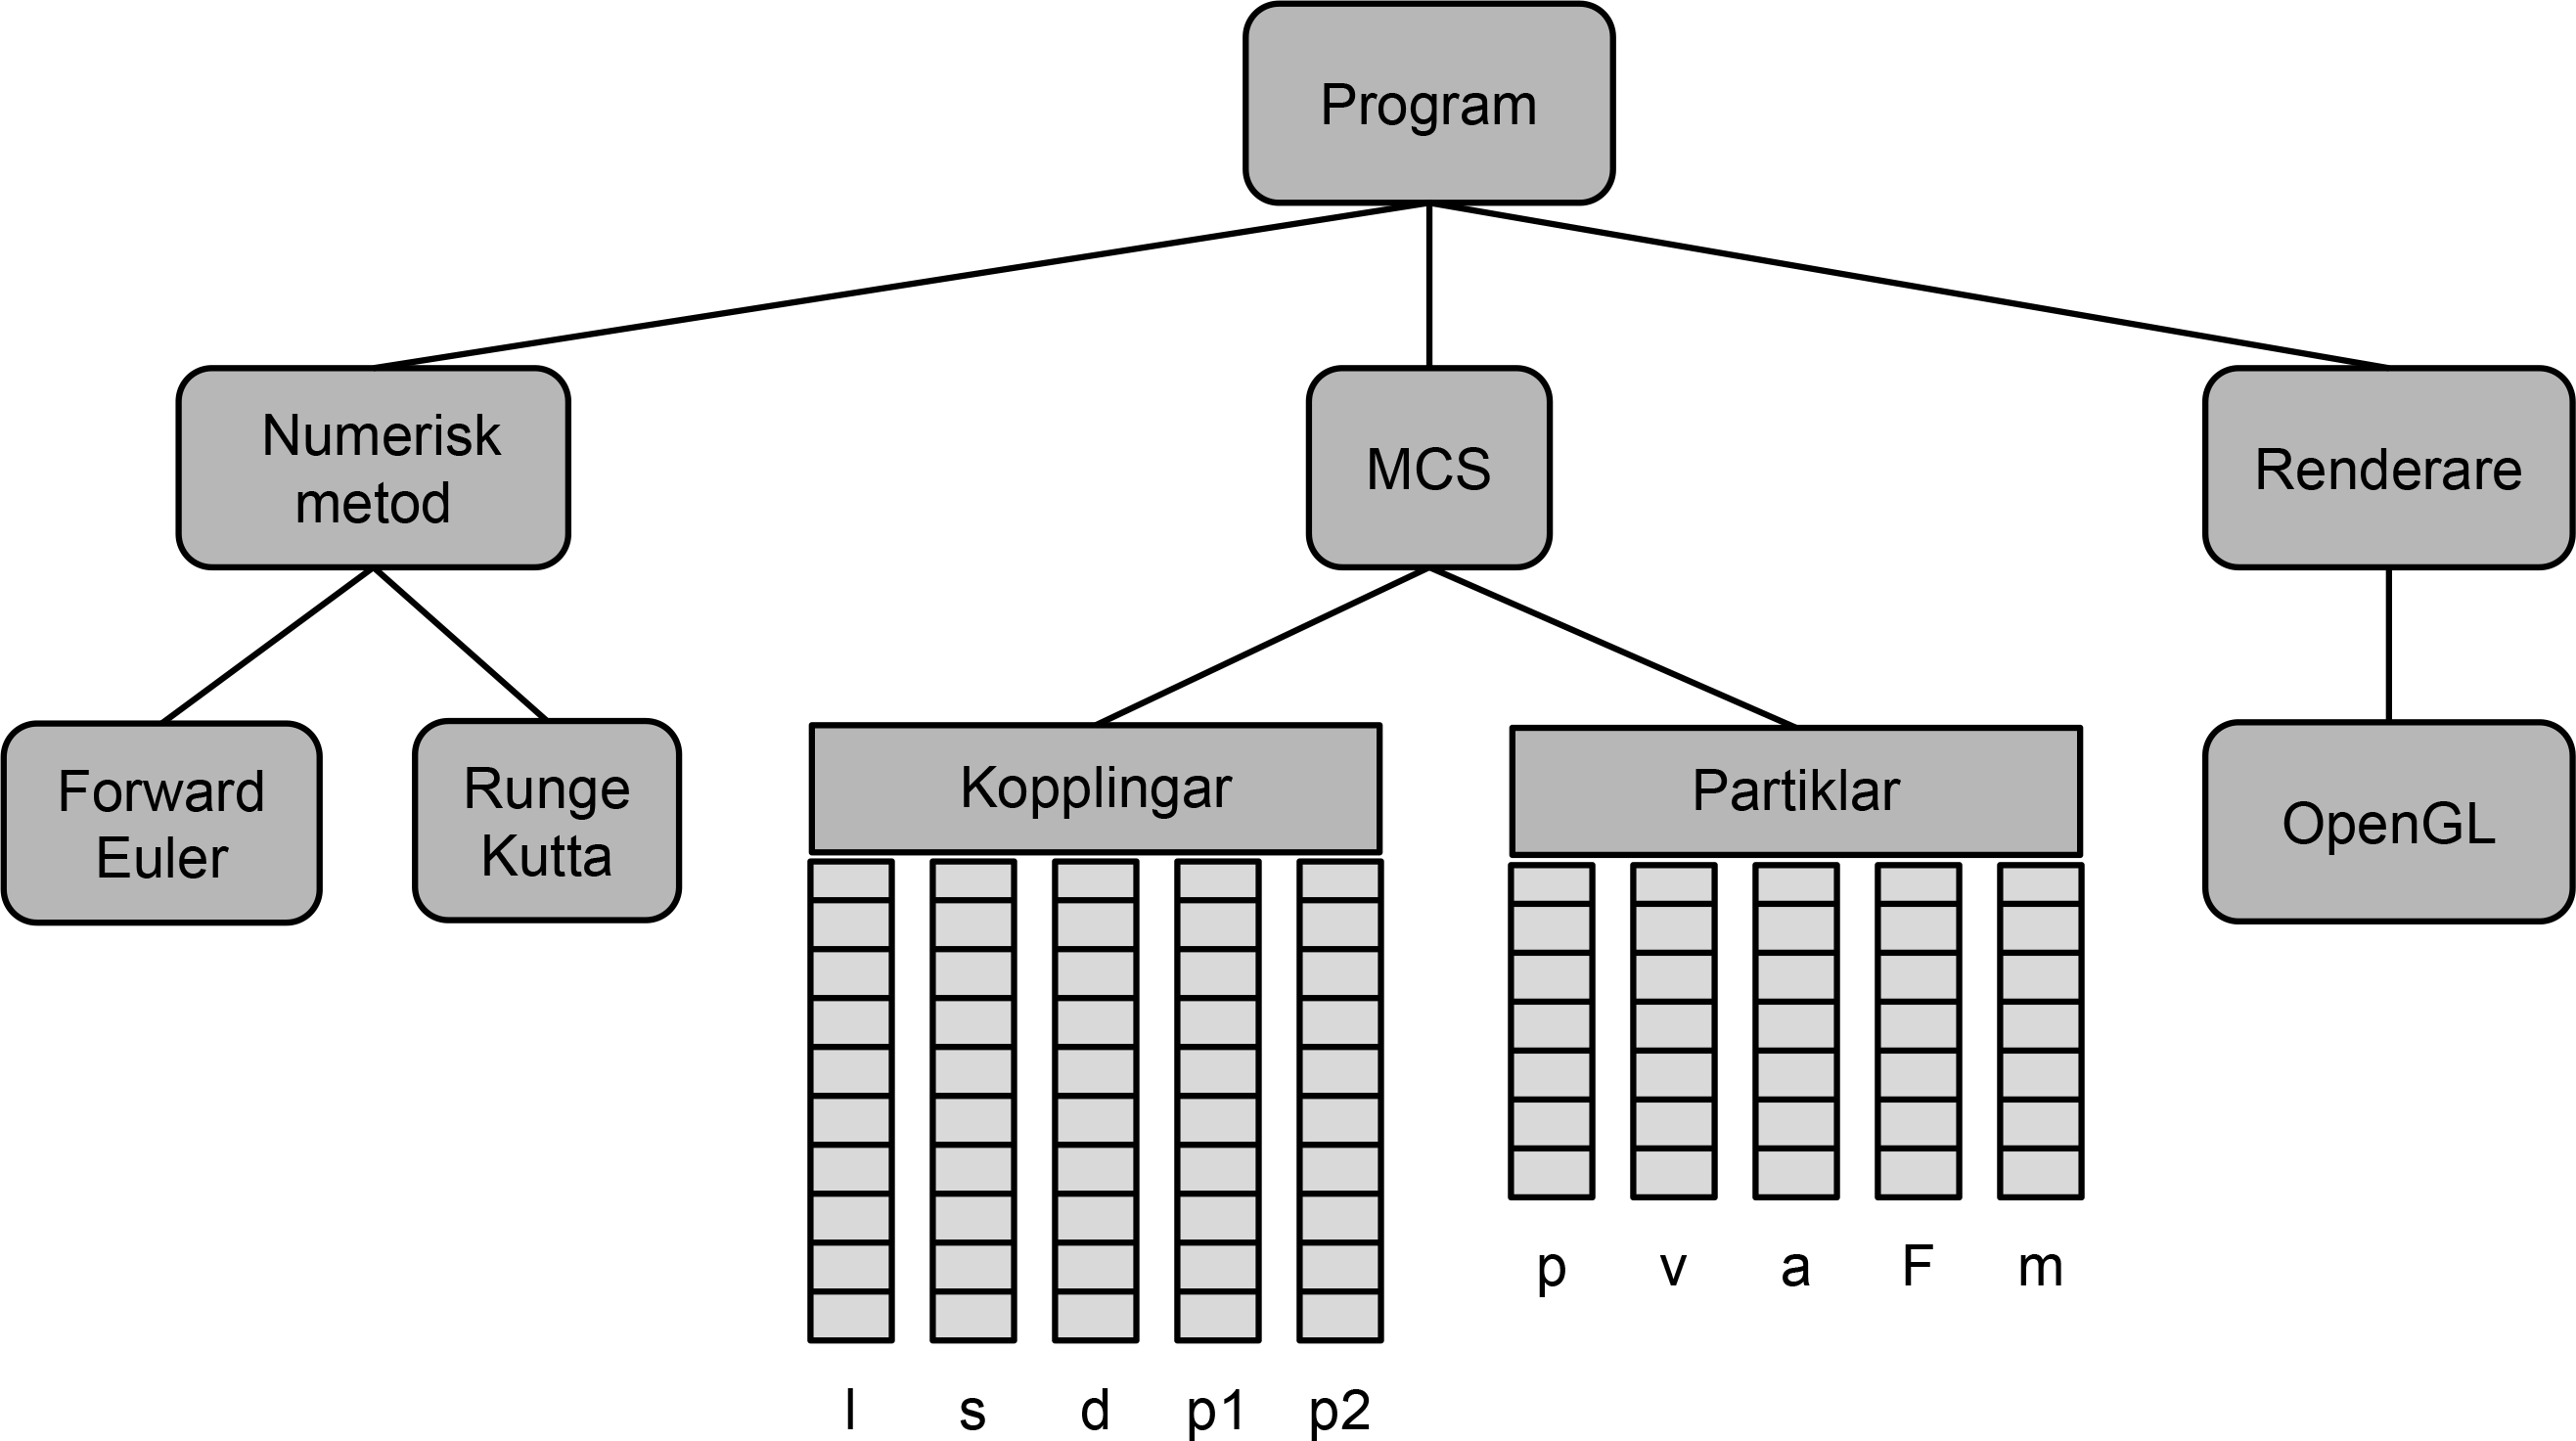
\includegraphics[width=16cm]{Bilder/Arkitektur.png} 
  \end{center}
  \caption{Övergripande systemarkitektur}
  \label{systemark}
\end{figure}
\\Klassen MCS (Mass Connection System) är den klass som lagrar all den huvudsakliga datan. 
Den innehåller samtliga partiklar och kopplingar för ett system.
\\\\Alla partiklar identifieras med ett index, och definieras av följande information:
\begin{itemize}
  \item p, position
  \item v, hastighet
  \item a, acceleration
  \item F, total momentan kraftpåverkan
  \item m, massa
\end{itemize}
Samtliga kopplingar identifieras med ett index, och definieras av följande information:
\begin{itemize}
  \item l, vilolängd
  \item k, fjäderkonstant
  \item b, dämparkonstant
  \item p1, index till den partikel som utgör kopplingens ena ändpunkt
  \item p2, index till den partikel som utgör kopplingens andra ändpunkt
\end{itemize}
Vad som också framgår i Figur Figur \ref{systemark} är att all numerisk integrering beräknas i en separat modul vilket gjorde det enkelt att ändra integreringsmetod vid behov, då den var oberoende av resten av systemet.

\subsubsection{Implementering av numeriska integreringsmetoder}
\paragraph{Eulers stegmetod} 
\paragraph{Runge Kutta}
\subsubsection{Rendering}
\subsection{Stabilitets- och prestandatest}


%Resultat
\section{Resultat}
\subsection{Resultat från förstudier}

\subsubsection{En dimension}
Resultatet från förstudierna i en dimension presenteras i Figur \ref{endim}. 
Här illustreras fem sammankopplade partiklars samverkan efter att en av dem har givits en förskjuten startposition. 
Den kraft som bildas av denna förskjutning kan ses påverka de andra partiklarna och fortplantas genom systemet över tid. 
Krafterna ses också dämpas och tillslut avta, vilket stabiliserar systemet.

\begin{figure}[h!]
  \begin{center}
    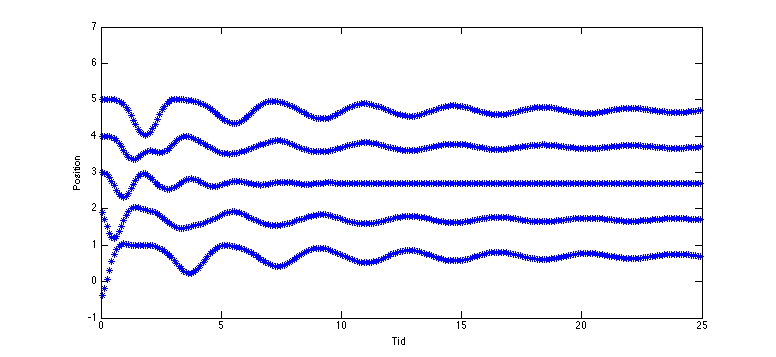
\includegraphics[width=16cm]{Bilder/1D_matlab.png} 
  \end{center}
  \caption{Endimensionellt MSD-system i MATLAB}
  \label{endim}
\end{figure}

\subsubsection{Två dimensioner}
I Figur \ref{tvådim} åskådliggörs resultatet av förstudierna i två dimensioner. 
Här illustreras ett 4x4 MSD-system som faller från sin startposition och därefter kolliderar med ett markplan.
Fjädrarnas inverkande krafter visualiseras genom att låta färgen bero på kopplingens längd. 
Kopplingen är grön i sitt viloläge och färgen går mot rött ju mer längden avviker från denna.

\begin{figure}[h!]
  \begin{center}
    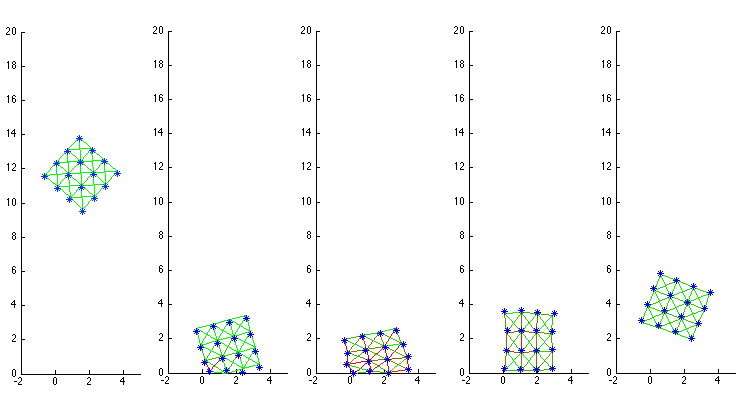
\includegraphics[width=16cm]{Bilder/boing.png} 
  \end{center}
  \caption{Tvådimensionellt 4x4 MSD-system i MATLAB}
  \label{tvådim}
\end{figure}

\subsection{Resultat från implementering}
\subsection{Resultat från stabilitets- och prestandatest}

%Diskussion
\section{Diskussion}


%Slutsats
\section{Slutsats}





%Referenser
\begin{thebibliography}{9}

\bibitem{pfleeger10softwareengineering}
Shari Lawrence Pfleeger och Joanne M. Atlee, \emph{Software Engineering, Fourth Edition, International Edition}, Pearson 2010
  
\end{thebibliography}

%Bilagor
\appendix

%Bilaga 1: Beskrivning av systemet
\section{Beskrivning av systemet}
\subsection{Systemkrav}
\subsubsection{Hårdvara}
\subsubsection{Mjukvara}

\subsection{Köra programmet}


\end{document}
